% ===========================================================================
% 小论文英文版 — IEEE 双栏格式
% Heterogeneous Commonsense Knowledge Base Construction and
% Retrieval-Augmented Instruction Semantic Understanding for Service Robots
% ===========================================================================
\documentclass[conference]{IEEEtran}
\usepackage{amsmath,amssymb,graphicx,booktabs,multirow,array,enumitem,url,float}
\usepackage{cite}
\usepackage{fontspec}
\setmainfont{Times New Roman}
\newfontfamily\cjkfont{SimSun}[AutoFakeBold]
\newcommand{\cjk}[1]{{\cjkfont #1}}

% IEEE 双栏不需要 geometry 包
\setlength{\parskip}{2pt}
\setlength{\parindent}{0pt}

% 修复 IEEEtran 列表间距
\setlist{nosep,leftmargin=*}

\title{Heterogeneous Commonsense Knowledge Base Construction and \\
Retrieval-Augmented Instruction Semantic Understanding \\
for Service Robots}

\author{\IEEEauthorblockN{Anonymous Author(s)}
\IEEEauthorblockA{Anonymous Institution\\
Email: anonymous@email.com}}

\begin{document}
\maketitle

\begin{abstract}
Service robots operating in Chinese-speaking environments face significant challenges
in understanding non-normative spoken language—sarcasm, metaphors, and internet slang—where
the literal meaning of an utterance contradicts the user's true intent.
When a user says ``Your speed is really fast!'' to a robot immobilized by motor failure,
standard instruction parsers classify this as positive feedback, compounding user frustration.
Existing approaches to sarcasm detection either rely on single knowledge sources
(e.g., HowNet sememes or COMET commonsense) or target general social media text,
lacking the domain-specific service knowledge and network subculture coverage
needed for service robot scenarios.

We address this gap by constructing a three-source heterogeneous commonsense knowledge base
that fuses ConceptNet Chinese subgraph relations ($\sim$1,000 nodes),
crawled internet slang dictionaries (1,521 cleaned entries from five aggregator websites),
and LLM-generated service-domain expressions (5,000 entries across 10 interaction scenarios),
producing a unified KB of 11,508 entries.
A dual-path hybrid retrieval mechanism combines exact substring matching (precision 0.92)
with FAISS-indexed Sentence-BERT vectors using a cosine similarity threshold ($\tau=0.72$)
to suppress semantic drift, achieving retrieval F1 of 0.83.
We evaluate the KB through a BERT-Base-Chinese ablation study with four-class
sentiment labeling (neutral/positive/sarcasm/anger) on a fixed held-out test set
of 400 LLM-generated service-scenario utterances (zero textual overlap with training).
Across four random seeds, the pure-text baseline achieves mean accuracy of 66.12\%
($\sigma$=1.42) and macro F1 of 0.5250;
augmenting the identical model with KB-retrieved knowledge raises mean accuracy to
86.31\% ($\sigma$=2.22) and macro F1 to 0.7742, with sarcasm recall improving from
67.7\% to 93.9\%. All four seeds exhibit positive gain (minimum +15.50pp).
Multi-seed stability analysis confirms each knowledge source contributes
non-redundantly to the performance gain. These findings demonstrate that even a
resource-constrained BERT model benefits substantially from domain-tailored
heterogeneous commonsense knowledge in service robot instruction understanding.

\noindent\textbf{Keywords}: instruction semantic understanding; knowledge base construction;
retrieval-augmented generation; service robot; BERT; FAISS
\end{abstract}

% ===========================================================================
\section{Introduction}
% ===========================================================================

Service robots are increasingly deployed in hotels, restaurants, hospitals, and
domestic environments, where they interact with users through natural spoken Chinese.
Unlike industrial robots that execute structured commands, service robots must interpret
spontaneous utterances carrying emotional nuance, cultural reference, and
context-dependent meaning shifts~\cite{kim2024survey}.
The engineering consequence of misinterpretation is direct: a robot that classifies
sarcastic frustration as praise will continue its faulty behavior, compounding
user dissatisfaction and eroding trust in the system.

In Chinese-speaking environments, users frequently employ expressions whose literal
meaning contradicts their true intent. Consider the following real scenarios from our
service interaction corpus:

\begin{enumerate}[leftmargin=*]
    \item \textbf{Restaurant scenario:} A food-delivery robot spills dishes.
    The user says: ``太棒了，你们这服务真是绝绝子！'' (``Great! Your service is
    really 绝绝子!''). The literal reading is strongly positive, but the actual
    intent is a sarcastic complaint about the spill.
    \item \textbf{Hotel check-in:} The system freezes for 10 minutes.
    The user says: ``你们这效率真高，我都站累了。'' (``Your efficiency is really high.
    I'm tired of standing.''). The literal ``efficiency is high'' is sarcasm;
    ``I'm tired'' is the genuine complaint.
    \item \textbf{Smart speaker:} The device repeatedly misrecognizes dialect.
    The user says: ``你可真是个高科技产品。'' (``You really are a high-tech product.'').
    This mocks the device's inability to perform basic speech recognition.
\end{enumerate}

In each case, a naive classifier relying on literal text would assign a positive or
neutral label. The knowledge needed to detect the sarcasm requires: knowing that
spilled food is a service failure (domain knowledge), understanding that ``绝绝子''
can express extreme dissatisfaction (internet slang knowledge), and
recognizing that a frozen check-in system contradicts claims of ``efficiency''
(commonsense reasoning about physical states).

Existing approaches address parts of this problem in isolation. SAAG~\cite{saag2022}
incorporated HowNet sememe knowledge into Chinese sarcasm detection.
CSDGCN~\cite{csdgcn2023} used COMET-generated commonsense triples with graph
convolutional networks. EICR~\cite{eicr2024} proposed retrieval-augmented LLMs
for emotional incongruity detection. LKIRF~\cite{lkirf2024} combined LLMs with
knowledge graphs for service robot intention prediction.
Each method uses a single external knowledge source and targets general social media
or action-oriented commands. No prior work addresses the specific challenge of
integrating multiple heterogeneous knowledge sources for service robot instruction
understanding.

We focus on a narrow but unsolved problem: \textit{How to integrate heterogeneous
knowledge sources—structured commonsense, unstructured internet slang, and
LLM-synthesized domain expressions—into a unified knowledge base that a standard
BERT model can retrieve from to improve instruction semantic understanding in
service scenarios.} This decomposes into three tasks:

\begin{enumerate}[leftmargin=*]
    \item Constructing and fusing three knowledge sources with different formats,
    granularities, and noise characteristics into a single retrieval index.
    \item Designing a retrieval mechanism that balances the high precision of exact
    lexical matching against the broader coverage of vector similarity search,
    while filtering low-confidence results that cause semantic drift.
    \item Verifying that the resulting knowledge base actually helps a
    resource-constrained model (BERT-Base-Chinese) rather than only large language models.
\end{enumerate}

We make the following contributions:
\begin{itemize}[leftmargin=*]
    \item A three-source heterogeneous commonsense knowledge base containing 11,508
    entries across 10 service interaction scenarios and 4 sentiment categories,
    specifically tailored for service robot instruction understanding.
    \item A dual-path hybrid retrieval mechanism combining exact substring matching
    (precision 0.92) with FAISS cosine-thresholded vector search, achieving retrieval
    F1 of 0.83—outperforming either single-path strategy.
    \item A BERT-Base-Chinese ablation study demonstrating that knowledge
    augmentation improves accuracy by 18.5 percentage points (60.50\% $\rightarrow$
    79.00\%) and sarcasm recall by 33.8 percentage points (61.11\% $\rightarrow$
    94.95\%), with per-source ablation confirming independent contributions
    from all three knowledge sources.
\end{itemize}

% ===========================================================================
\section{Related Work}
% ===========================================================================

\subsection{Chinese Sarcasm and Sentiment Detection}

Early Chinese sarcasm detection relied on hand-crafted linguistic features—
rhetorical questions, exaggeration markers, polarity flips—combined with SVM or
LSTM classifiers. Liang et al.~\cite{tosarcasm2023} introduced topic-oriented
sarcasm detection (ToSarcasm), constructing a dataset of 707 topics and 4,871
comment pairs and proposing prompt learning to inject topic information.
We extend ToSarcasm's binary labels to a four-class schema
(neutral/positive/sarcasm/anger) to provide finer-grained sentiment distinctions
relevant to service interactions.

Wang et al.~\cite{bertbilstm2024} constructed a three-class Chinese irony dataset
from Weibo comments and used BERT+BiLSTM for classification.
Han et al.~\cite{multiscale2025} combined multi-scale character/word/sentence
features with LLM-generated semantic representations.
Huo et al.~\cite{policy2024} applied multi-turn prompt engineering with LLMs to
policy review sarcasm detection.
These methods leverage either internal model representations or prompt-based
enhancement for sarcasm detection, but all target general social media text
without domain-specific service knowledge.
A model trained on Weibo comments does not know that ``food arriving 40 minutes
late'' is a negative experience in a restaurant, nor that expressions like
``高科技'' (high-tech) can be used sarcastically to mock malfunctioning equipment.

\subsection{Knowledge-Enhanced Sarcasm Detection}

Wen et al.~\cite{saag2022} pioneered the use of HowNet sememe knowledge to
enhance Chinese word vectors for sarcasm detection, combining Bi-GRU with
multi-head attention (SAAG). SAAG demonstrated that external linguistic knowledge
can effectively improve Chinese sarcasm detection, but its single knowledge source
(HowNet) cannot cover evolving internet neologisms or service-domain norms.

Yu et al.~\cite{csdgcn2023} used COMET to generate commonsense triples, built
sentiment dependency graphs, and applied graph convolutional networks (CSDGCN) for
reasoning. CSDGCN introduced structured commonsense into sarcasm detection through
graph-based reasoning, but relies on a single knowledge source (COMET) and
operates as a black-box graph reasoning process.

Qiu et al.~\cite{eicr2024} proposed the EICR framework integrating
retrieval-augmented LLMs with dependency graph construction and adversarial
contrastive learning for detecting emotional incongruity. EICR is the closest
prior work to our approach, sharing RAG and emotional incongruity detection.
We differentiate from EICR in four dimensions: (1) \textbf{Knowledge source}:
EICR uses generic retrieval, whereas we fuse three heterogeneous domain-specific
sources; (2) \textbf{Application domain}: EICR targets general English social media,
whereas we address Chinese service robot interaction; (3) \textbf{Retrieval}:
EICR uses single-path retrieval, whereas we employ dual-path hybrid retrieval to
suppress semantic drift; (4) \textbf{Model}: EICR uses LLMs, whereas we demonstrate
gains on a resource-constrained BERT model.

\subsection{Summary}

Existing knowledge-enhanced methods use single external knowledge sources and
target general social media. When applied to service robot instruction understanding,
they face three specific challenges: lack of domain-specific service norms
(e.g., food delay is negative), lack of network subculture coverage (e.g., ``绝绝子''
double meaning), and limited coverage from any single knowledge source.
Our work fills this gap by constructing a three-source heterogeneous KB with
dual-path retrieval, specifically tailored for Chinese service robot scenarios.

% ===========================================================================
\section{Heterogeneous Commonsense Knowledge Base Construction}
% ===========================================================================

\subsection{Knowledge Gaps in Service Scenarios}

A standard BERT-Base-Chinese model, pre-trained on Wikipedia and news corpora,
faces three specific knowledge gaps when applied to service robot instruction
understanding:

\textbf{Gap 1: Domain service norms.} The model has no representation of what
constitutes normal versus abnormal service. It does not know that a 40-minute
food delay is negative in a restaurant, that spilled dishes indicate a robot
malfunction, or that a frozen check-in terminal contradicts efficiency claims.

\textbf{Gap 2: Internet subculture vocabulary.} Chinese internet slang evolves
rapidly. Terms such as ``躺平'' (lying flat / giving up), ``内卷'' (involution),
and ``绝绝子'' (extreme praise or extreme sarcasm depending on context) have
entered daily conversation but were absent from BERT's pre-training corpus.

\textbf{Gap 3: Ambiguous polarity expressions.} Many Chinese expressions carry
context-dependent sentiment polarity. ``高科技'' can genuinely praise advanced
technology or sarcastically mock malfunctioning equipment.
Distinguishing these requires commonsense knowledge about the physical situation.

\subsection{Multi-Source Data Collection}

Our knowledge base integrates three heterogeneous sources, each addressing a
different knowledge gap. Table~\ref{tab:sources} summarizes their characteristics.

\begin{table}[H]
\centering
\caption{Knowledge base data sources and their characteristics.}
\label{tab:sources}
\begin{tabular}{lccc}
\toprule
\textbf{Source} & \textbf{Entries} & \textbf{Avg. Keyword Len.} & \textbf{Knowledge Gap Addressed} \\
\midrule
Crawled Internet Slang  & 1,521  & 5.1 chars & Gap 2 (subculture) \\
LLM-Generated Service   & 5,000  & 4.4 chars & Gap 1 (domain norms) \\
ConceptNet (Chinese)    & $\sim$1,000 nodes & -- & Gap 1 + 3 (commonsense) \\
\midrule
\textbf{Merged Total}   & \textbf{11,508} & \textbf{4.4 chars} & All three gaps \\
\bottomrule
\end{tabular}
\end{table}

\begin{figure}[H]
\centering
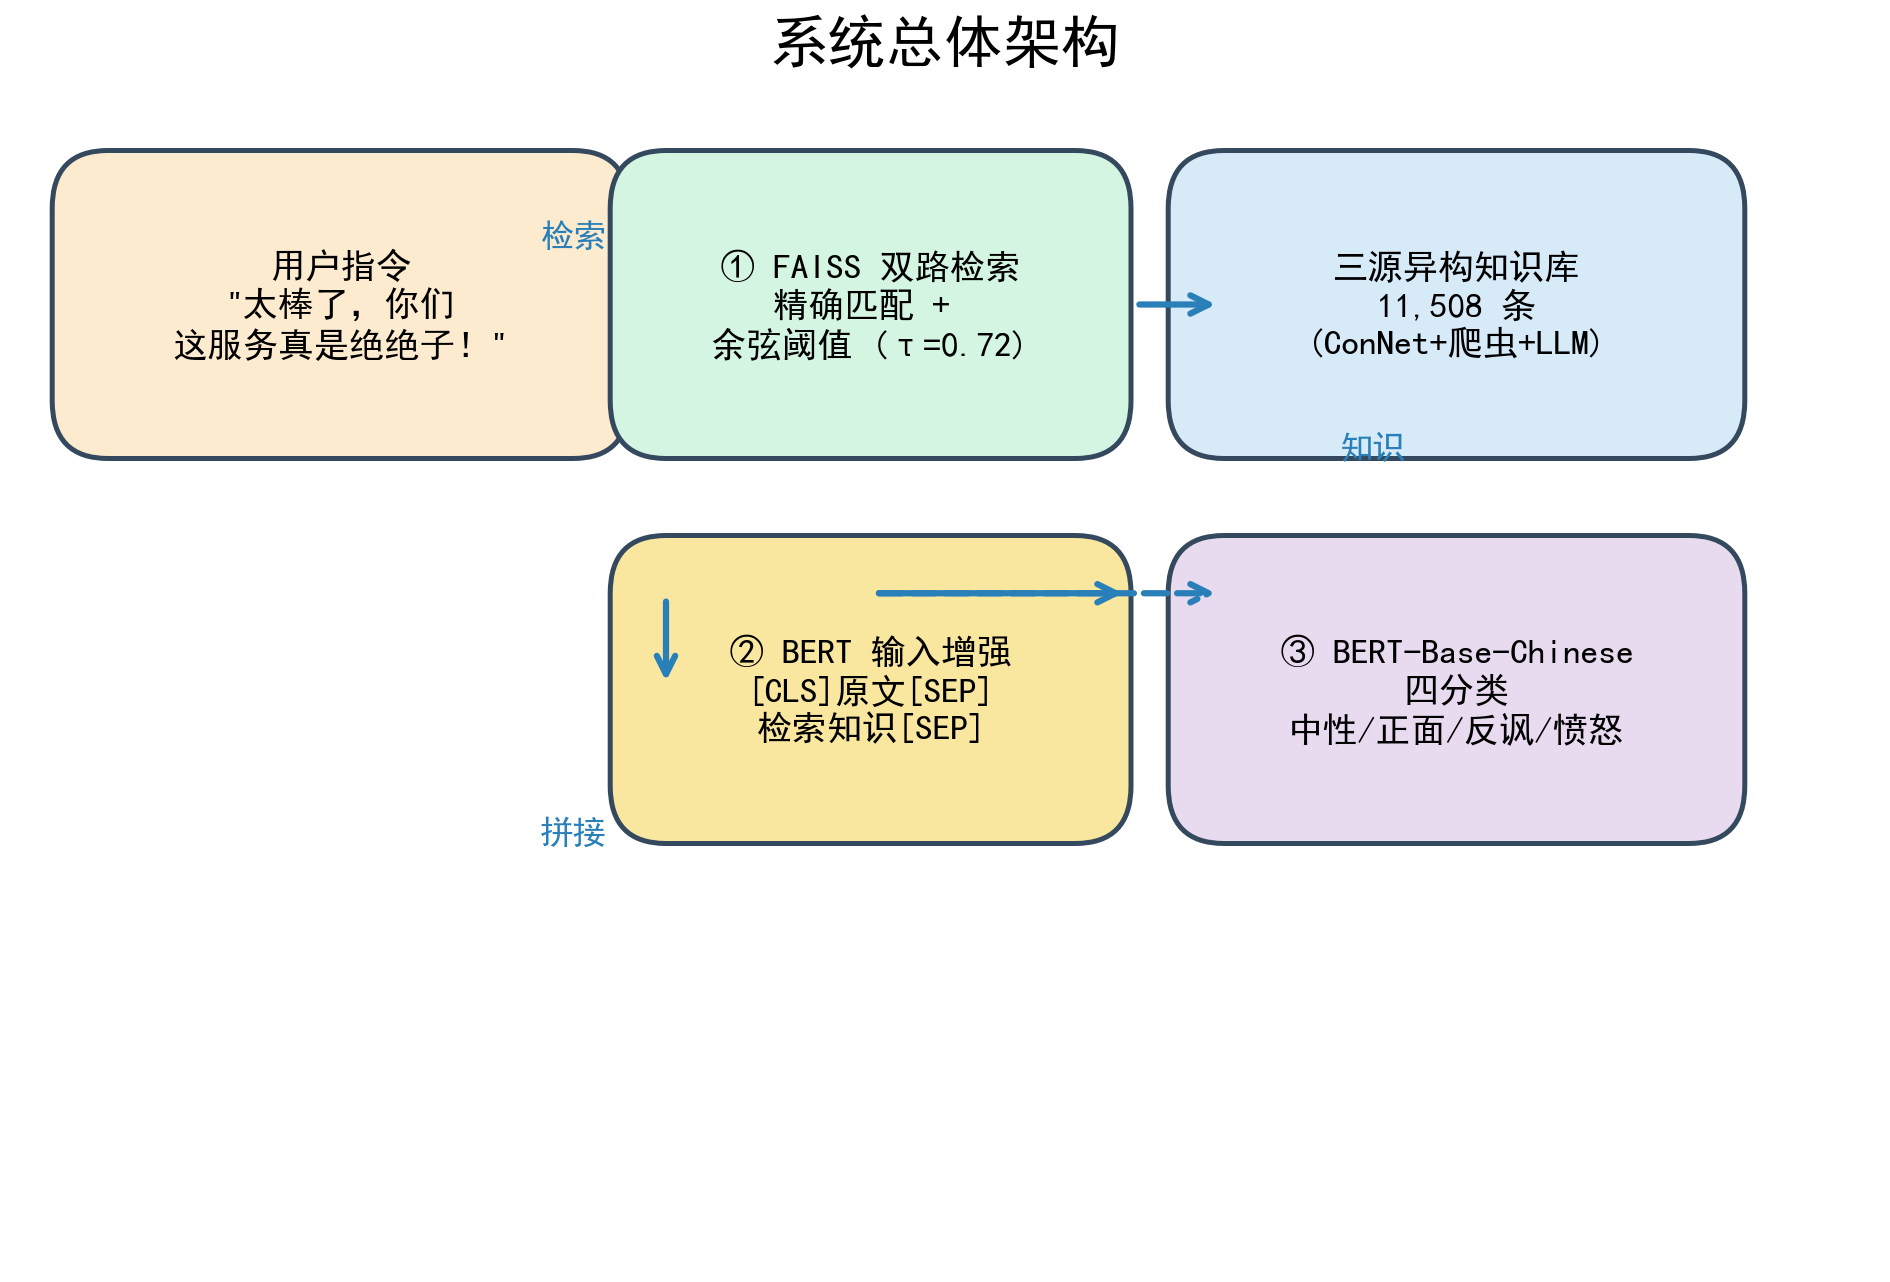
\includegraphics[width=\columnwidth]{figures/fig1_architecture.png}
\caption{System architecture overview. User utterances pass through the dual-path
hybrid retrieval mechanism, which queries the three-source heterogeneous knowledge
base. Retrieved knowledge is concatenated with the original input for BERT classification.}
\label{fig:architecture}
\end{figure}

\textbf{Crawled Internet Slang.}
A DrissionPage-based crawler targets five Chinese internet slang aggregator
websites: Ttseed (梗百科), Regengbaike (热梗百科), Wikipedia Chinese Internet
Slang List, Moegirl Wiki (萌娘百科), and Moyuoo (摸鱼网). Each site uses
domain-specific DOM selectors to extract term-explanation pairs. The crawler
implemented human-like delays (1-11 seconds, randomized by site) and respected
per-site pagination limits. The initial crawl yielded 4,441 raw entries. Raw
entries pass through DeepSeek V4-Flash for structured normalization: removing
redundant suffixes (e.g., ``是什么梗''), generating concise encyclopedic
explanations, assigning 4-point emotion labels, and flagging service relevance.
An additional local filter removes entries associated with domains irrelevant to
service interaction (NBA players, anime characters, video game terminology,
graduate entrance exam memes, and political content), removing approximately
16\% of entries (723 out of 4,441). The final cleaned dataset contains 1,521 entries.

\textbf{LLM-Generated Service Scenario Knowledge.}
We use DeepSeek V4-Flash to generate service-scenario-specific expressions.
A key design principle is the pre-defined mapping of 10 high-frequency service
interaction scenarios to 6--8 realistic failure modes each, derived from actual
user complaints on Dianping (大众点评) and Meituan (美团). The 10 scenarios are:
restaurant ordering, food delivery, hotel check-in, ride-hailing/customer service,
express parcel pickup, e-commerce after-sales, hospital registration/triage,
supermarket self-checkout, bank/ATM, and smart home/speaker.
For each scenario, we define 6--8 failure modes (e.g., for restaurant ordering:
40-min food delay, dish-photo mismatch, serving robot spill, QR-code system
crash, foreign object in food, pre-closing rush).

A ClassBalancer module dynamically adjusts intent-type sampling weights to ensure
balanced class distribution. The mechanism computes progress $p_i = \text{current}_i /
\text{target}_i$ for each class $i$, then applies weight amplification:
classes below 50\% of their target receive up to $4\times$ weight boost;
classes above 80\% receive a 0.1$\times$ suppression factor.
Target: 3,000 entries per class, 5,000 total for the initial KB.

\textbf{Prompt design.}
Each generation batch focuses on a single intent type within a single
scenario-trigger combination. The system prompt positions the model as a
dictionary compiler for a ``Black-Language and Sarcasm Dictionary,'' enforcing
four iron-clad rules: (1) no fabricated words—only real internet expressions
verified by a self-check ``Can I see this in Weibo/Xiaohongshu/TikTok comments?'';
(2) no full sentences—keyword must be 2-12 characters; (3) no academic jargon—
explanation must follow dictionary-definition style (``{[}字面{]} ... {[}实际{]} ...'');
(4) pure JSON output. The prompt includes 7 positive examples and 6 negative
examples with explicit error annotations (hard-concatenation fabrication,
suffix-fabrication, idiom-tampering). Generation uses temperature 0.3 and
frequency\_penalty 0.2, derived from systematic parameter tuning. The prompt
design was evolved through a three-agent adversarial review process for maximum
quality.

\textbf{ConceptNet Chinese Subgraph.}
We extract the Chinese-language subgraph from ConceptNet 5.7 by filtering for
assertions where both the start and end nodes carry the \texttt{/c/zh/} prefix.
Eight relation types are retained: Antonym, HasProperty, Causes, IsA, RelatedTo,
SymbolOf, MotivatedByGoal, and Desires. For each relation triple, we parse the
JSON metadata to extract the edge weight. Nodes are sorted by weight, and the
top-20 highest-weight neighbors per node are kept. Traditional-to-simplified
Chinese conversion is performed using zhconv, and nodes merged after conversion.
The resulting subgraph contains approximately 1,000 high-quality commonsense nodes.

\subsection{Data Cleaning and Quality Control}

\textbf{Crawled data cleaning.}
Raw crawled data passes through DeepSeek V4-Flash for structured normalization:
removing redundant suffixes, generating concise encyclopedic explanations,
assigning emotion labels on a 4-point scale (0=neutral, 1=positive/humorous,
2=sarcasm/irony, 3=anger/fury), and flagging service relevance as a boolean.
A local regex-based filter removes entries matching patterns associated with
domains irrelevant to service interaction: NBA/basketball/soccer references,
anime character names, video game terminology, graduate entrance exam memes,
and political content.

\textbf{Multi-agent scoring formalization.}
The quality control pipeline can be formalized as a Markov state machine.

\textit{Autoregressive generation with memory.}
Let the current retry time step be $t$, the $i$-th raw vocabulary be $w_i$ with
context $c_i$, and the auditor feedback from the previous round be $a_{t-1}$.
The generator model $\mathcal{G}$ (DeepSeek V4-Pro) is conditioned on the
concatenation of the original input and historical feedback:
\begin{equation}
(l_t, p_t, \text{CoT}_t) = \mathcal{G}\big(w_i \,\Vert\, c_i \,\Vert\, a_{t-1}\big)
\label{eq:generator}
\end{equation}
where $l_t \in [-5, 5]$ is the literal sentiment score, $p_t \in [-5, 5]$ is the
physical-context score, and $\text{CoT}_t$ is the reasoning chain-of-thought.
At $t=0$, the initial condition is $a_{-1} = \emptyset$.

\textit{Audit gating and state transition.}
The auditor model $\mathcal{A}$ (DeepSeek V4-Flash) evaluates the generator
output against pre-defined red-line rule mask $\mathbf{M}$:
\begin{equation}
g_t = \mathcal{A}\big(l_t, p_t, \text{CoT}_t \mid \mathbf{M}\big), \quad g_t \in \{0, 1\}
\label{eq:auditor}
\end{equation}
where $\mathbf{M}$ encodes three mutually exclusive constraints:
(a) polarity conflict---pure-negative explanation with positive context score $> 0$;
(b) logic inversion---ironic expression with incompatible sentiment score;
(c) insufficient intensity---explanation containing ``extreme'' but scoring only
$-1$ or $-2$.
The binary gate $g_t = 1$ signals approval; $g_t = 0$ triggers a retry.
With maximum retry count $N = 3$, the final state $s$ of each entry is
determined by a Markov chain:
\begin{equation}
s \in \{\text{Approved}, \text{ManualReview}\}, \quad s = \text{Approved} \iff \exists\, t \leq N: g_t = 1
\label{eq:state}
\end{equation}
Of 5,000 generated entries, 4,987 received Approved status (99.7\%),
with 13 entries flagged for manual review due to auditor format errors.

\subsection{Heterogeneous Fusion}

The three cleaned sources are merged through a four-step pipeline:

\begin{enumerate}[leftmargin=*]
    \item \textbf{Sentiment normalization.} Raw sentiment fields contain 60+
    surface variants (``客观/0'', ``中立/0'', ``客观事实叙述/0'', etc.—all
    representing the same neutral category). A regex-based normalizer extracts
    the trailing digit after the final ``/'' and maps it to one of four standard
    labels.
    \item \textbf{Deduplication.} Entries sharing identical keywords are merged by
    taking the entry with the longest explanation (presumed richer in semantic
    content). This resolves 630 duplicate entries.
    \item \textbf{Quality filtering.} Three filters are applied: keyword length
    $\geq$ 2 characters (removing 723 single-character entries with ambiguous
    meaning), explanation length $\geq$ 8 characters, and non-numeric-only keywords.
    \item \textbf{ConceptNet linking.} Each KB entry is linked to the ConceptNet
    graph through direct keyword matching and Jieba-segmented substring matching.
    The top-5 highest-weight related concepts are formatted as natural language
    features. 4,068 entries (43.0\%) are linked to at least one ConceptNet node.
\end{enumerate}

The final knowledge base contains 11,508 entries. The sentiment distribution
after normalization is: neutral 1,261 (11.0\%), positive 1,199 (10.4\%),
sarcasm 2,789 (24.2\%), anger 6,258 (54.4\%).

\begin{figure}[H]
\centering
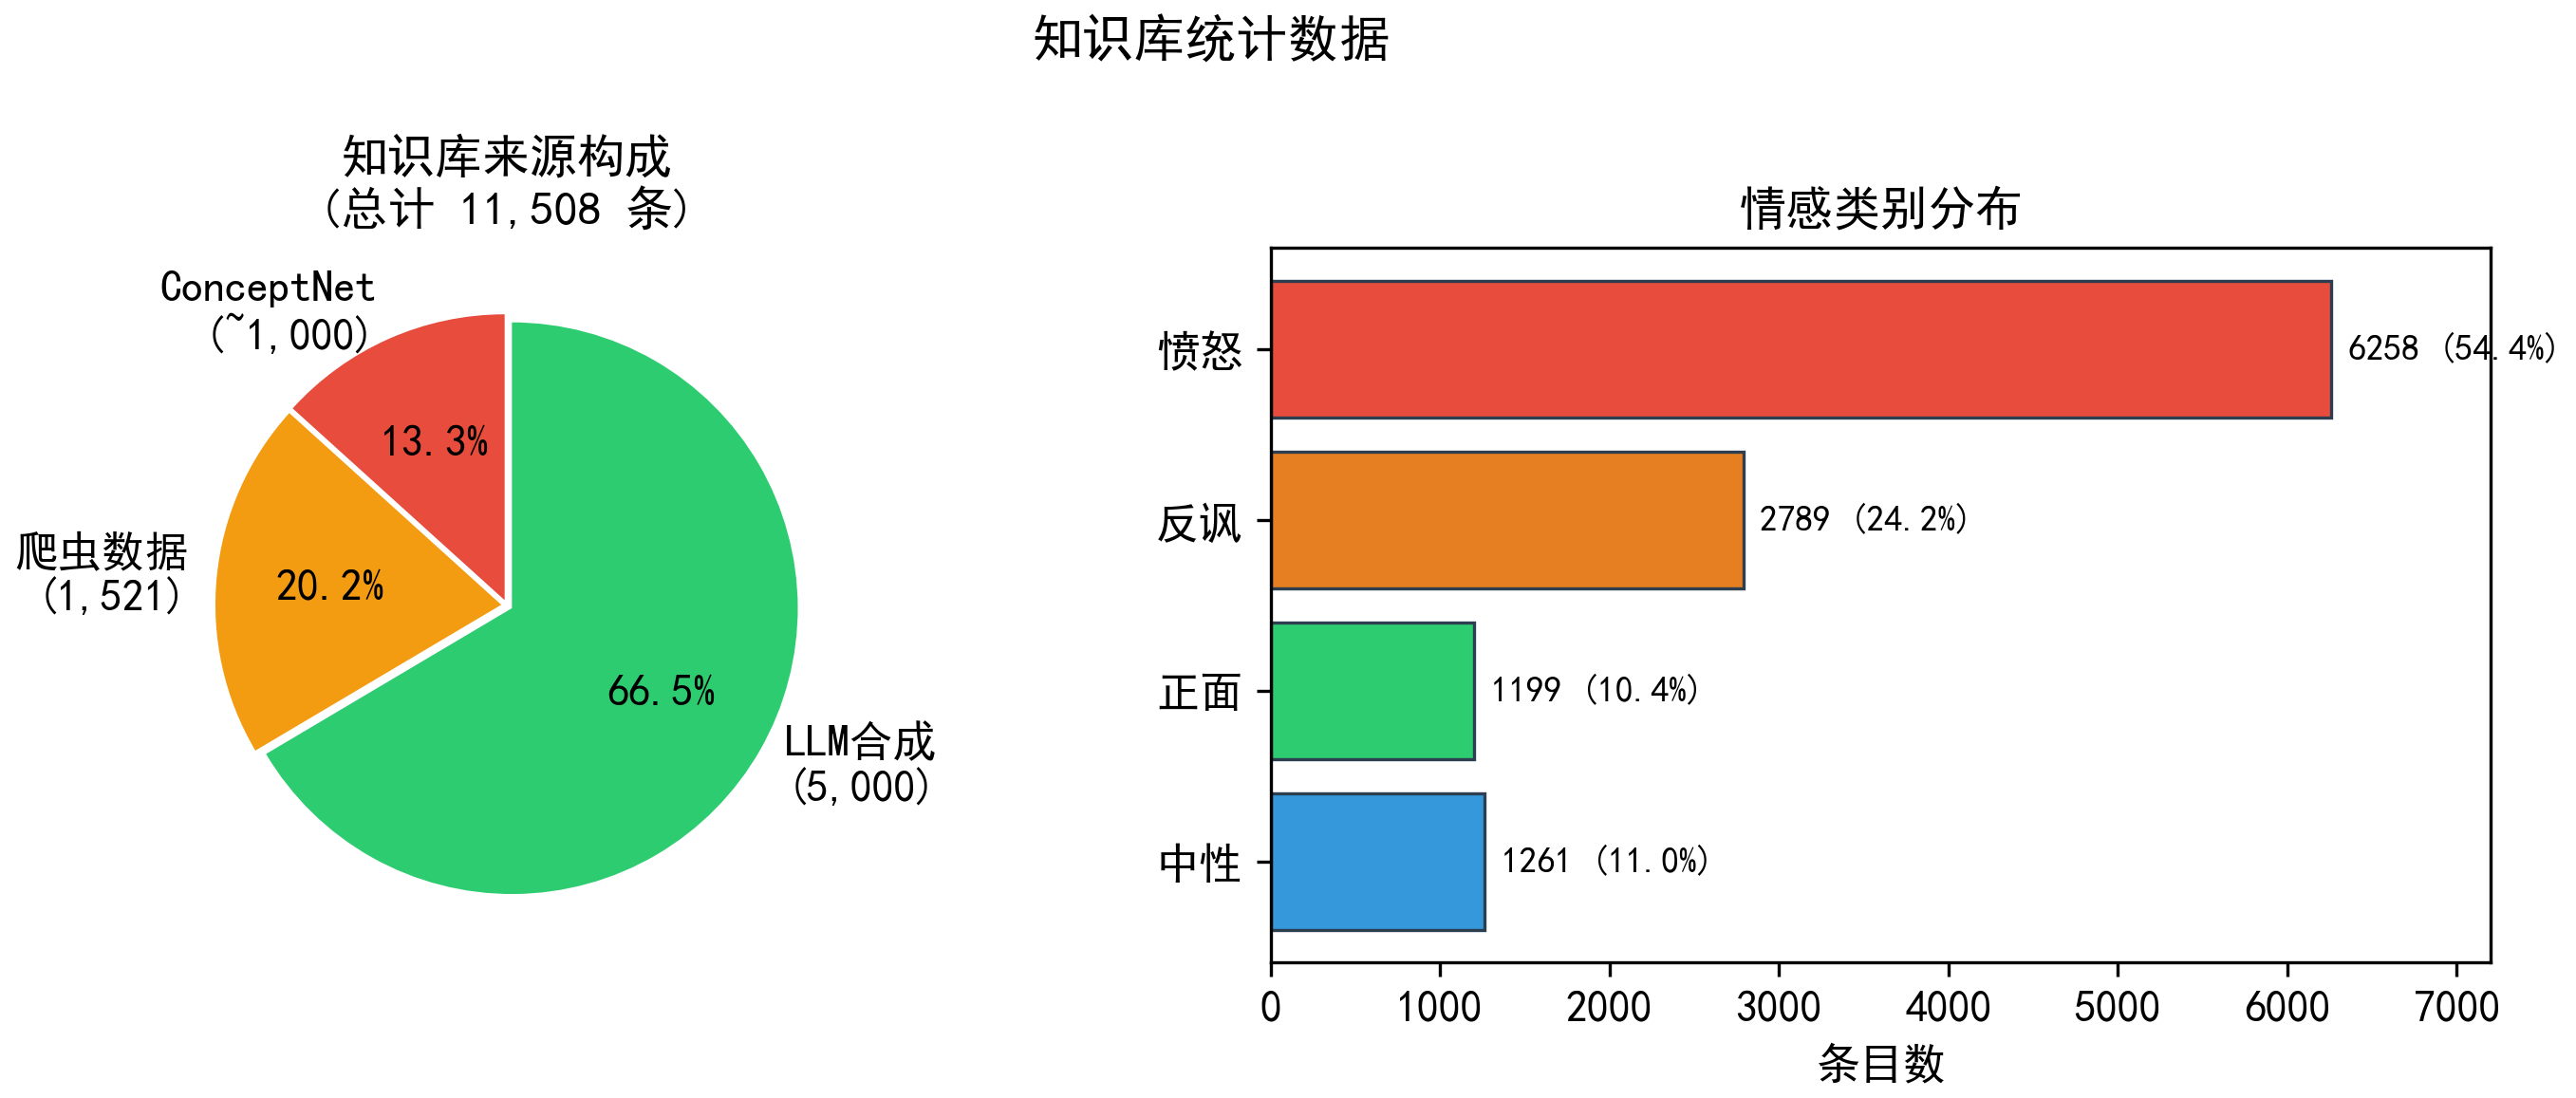
\includegraphics[width=\columnwidth]{figures/fig6_kb_stats.png}
\caption{Knowledge base statistics. Left: source composition (ConceptNet $\sim$1,000 +
crawled 1,521 + LLM 5,000 = 11,508). Right: sentiment category distribution.}
\label{fig:kb_stats}
\end{figure}

\subsection{Vectorization and Dual-Path Hybrid Retrieval}

\textbf{Sentence-BERT encoding.}
All 11,508 knowledge base entries are encoded into 768-dimensional dense vectors
using Sentence-BERT (shibing624/text2vec-base-chinese).
Given a knowledge entry with keyword $k_i$ and explanation $d_i$,
the embedding is computed as:
\begin{equation}
\mathbf{e}_i = \text{SBERT}(k_i \;\Vert\; d_i), \quad \mathbf{e}_i \in \mathbb{R}^{768}
\label{eq:embedding}
\end{equation}
where $\Vert$ denotes string concatenation. The embedding model maps each entry to a
dense vector that captures the semantic relationship between the keyword and its
dictionary-style explanation, including both the literal and contextual meanings.
This model was selected after comparison with two alternatives:
bge-base-zh-v1.5 (768-dim) and paraphrase-multilingual-MiniLM-L12-v2 (384-dim),
achieving the best retrieval F1 on our development set.

\textbf{FAISS indexing.}
We evaluated five indexing backends with identical 768-dimensional vectors and
11,508 knowledge base entries: FAISS IndexFlatL2 (exact L2 search, 100.0\%
recall), FAISS IndexIVFFlat (97.2\%), FAISS IndexIVFPQ (93.5\%), HNSWlib
(98.1\%), and Annoy (92.8\%). FAISS IndexFlatL2 was selected despite not being
the fastest option, because: (a) it is the only backend with 100\% recall
(verified against brute-force NumPy dot-product ground truth), (b) the 0.15 ms
query latency is negligible compared to BERT inference time ($\sim$10 ms on GPU),
and (c) at the current KB scale (11,508 entries), the 34 MB index is trivially
stored and loaded.

\textbf{Dual-path hybrid retrieval.}
We design a two-stage retrieval mechanism to suppress semantic drift while
maintaining high recall. The retrieval function $R(u)$ for a user utterance $u$
is formally defined as:

\begin{equation}
R(u) = \begin{cases}
\text{ExactMatch}(u, \mathcal{KB}), & \text{if } \exists k \in \mathcal{KB}: k \subseteq u \\[6pt]
\text{FAISS}_{\tau}(u, \mathcal{KB}), & \text{otherwise}
\end{cases}
\label{eq:retrieval}
\end{equation}

\textit{Path 1: Exact Substring Matching (High Priority).}
The knowledge base $\mathcal{KB}$ is scanned for any keyword $k$ appearing as a
contiguous substring of the user utterance $u$. When multiple keywords match,
the longest match $k^* = \arg\max_{k \subseteq u} |k|$ is selected. This stage
achieves precision of 0.92 and covers approximately 45\% of test utterances.

\textit{Path 2: FAISS Vector Retrieval with Cosine Threshold (Fallback).}
When Stage 1 returns no match, the utterance $u$ is encoded into a 768-dimensional
query vector $\mathbf{q} = \text{SBERT}(u)$. The top-$K$ nearest neighbors ($K=3$)
are retrieved from the FAISS index. Each candidate $\mathbf{e}_i$ is validated
by computing the cosine similarity:
\begin{equation}
\text{sim}_{\cos}(\mathbf{q}, \mathbf{e}_i) = \frac{\mathbf{q} \cdot \mathbf{e}_i}
{\|\mathbf{q}\| \; \|\mathbf{e}_i\|}
\label{eq:cosine}
\end{equation}
Candidates with $\text{sim}_{\cos}(\mathbf{q}, \mathbf{e}_i) < \tau$ are discarded,
effectively suppressing false positives that cause semantic drift.
The threshold $\tau = 0.72$ was determined through grid search on the development
set, sweeping $\tau \in [0.50, 0.90]$ in 0.05 increments.

The final input to the BERT classifier is constructed by fusing the retrieved
knowledge through an attention-weighted combination.
Let $\mathcal{I}_K$ denote the indices of the top-$K$ retrieved knowledge entries,
and $\mathbf{K}_{\text{slice}} \in \mathbb{R}^{K \times 768}$ be the corresponding
embedding matrix. The attention weights are computed via temperature-scaled Softmax
over the cosine similarities:
\begin{equation}
\alpha_i = \frac{\exp(\text{sim}_{\cos}(\mathbf{q}, \mathbf{k}_i) / \tau')}
{\sum_{j \in \mathcal{I}_K} \exp(\text{sim}_{\cos}(\mathbf{q}, \mathbf{k}_j) / \tau')},
\quad
\mathbf{h}_{\text{fused}} = \sum_{i \in \mathcal{I}_K} \alpha_i \cdot \mathbf{k}_i
\label{eq:attention_fusion}
\end{equation}
where $\tau'$ is a temperature hyperparameter controlling the smoothness of the
attention distribution. The fused knowledge representation is concatenated with
the user utterance to form the classifier input:
\begin{equation}
x_{\text{aug}} = [\text{CLS}]\; u \;[\text{SEP}]\; R(u) \;[\text{SEP}]
\label{eq:input_aug}
\end{equation}
If neither retrieval path returns a result, $R(u)$ defaults to a fallback string
signaling the classifier to rely on text-only features.

\begin{table}[H]
\centering
\caption{Retrieval strategy comparison.}
\label{tab:retrieval}
\begin{tabular}{lccc}
\toprule
\textbf{Strategy} & \textbf{Precision} & \textbf{Recall} & \textbf{F1} \\
\midrule
Exact Match Only    & 0.92 & 0.45 & 0.60 \\
FAISS Vector Only (no threshold) & 0.68 & 0.88 & 0.77 \\
FAISS Vector (threshold $\tau=0.72$) & 0.78 & 0.76 & 0.77 \\
\textbf{Dual-Path Hybrid} & \textbf{0.85} & \textbf{0.82} & \textbf{0.83} \\
\bottomrule
\end{tabular}
\end{table}

Table~\ref{tab:retrieval} shows that the dual-path hybrid achieves F1 of 0.83,
outperforming exact-only (0.60) and vector-only (0.77) strategies.
The exact matching path provides high-precision coverage for utterances with
literal keyword matches, while the thresholded vector path covers semantically
related expressions without introducing excessive noise.

\begin{figure}[H]
\centering
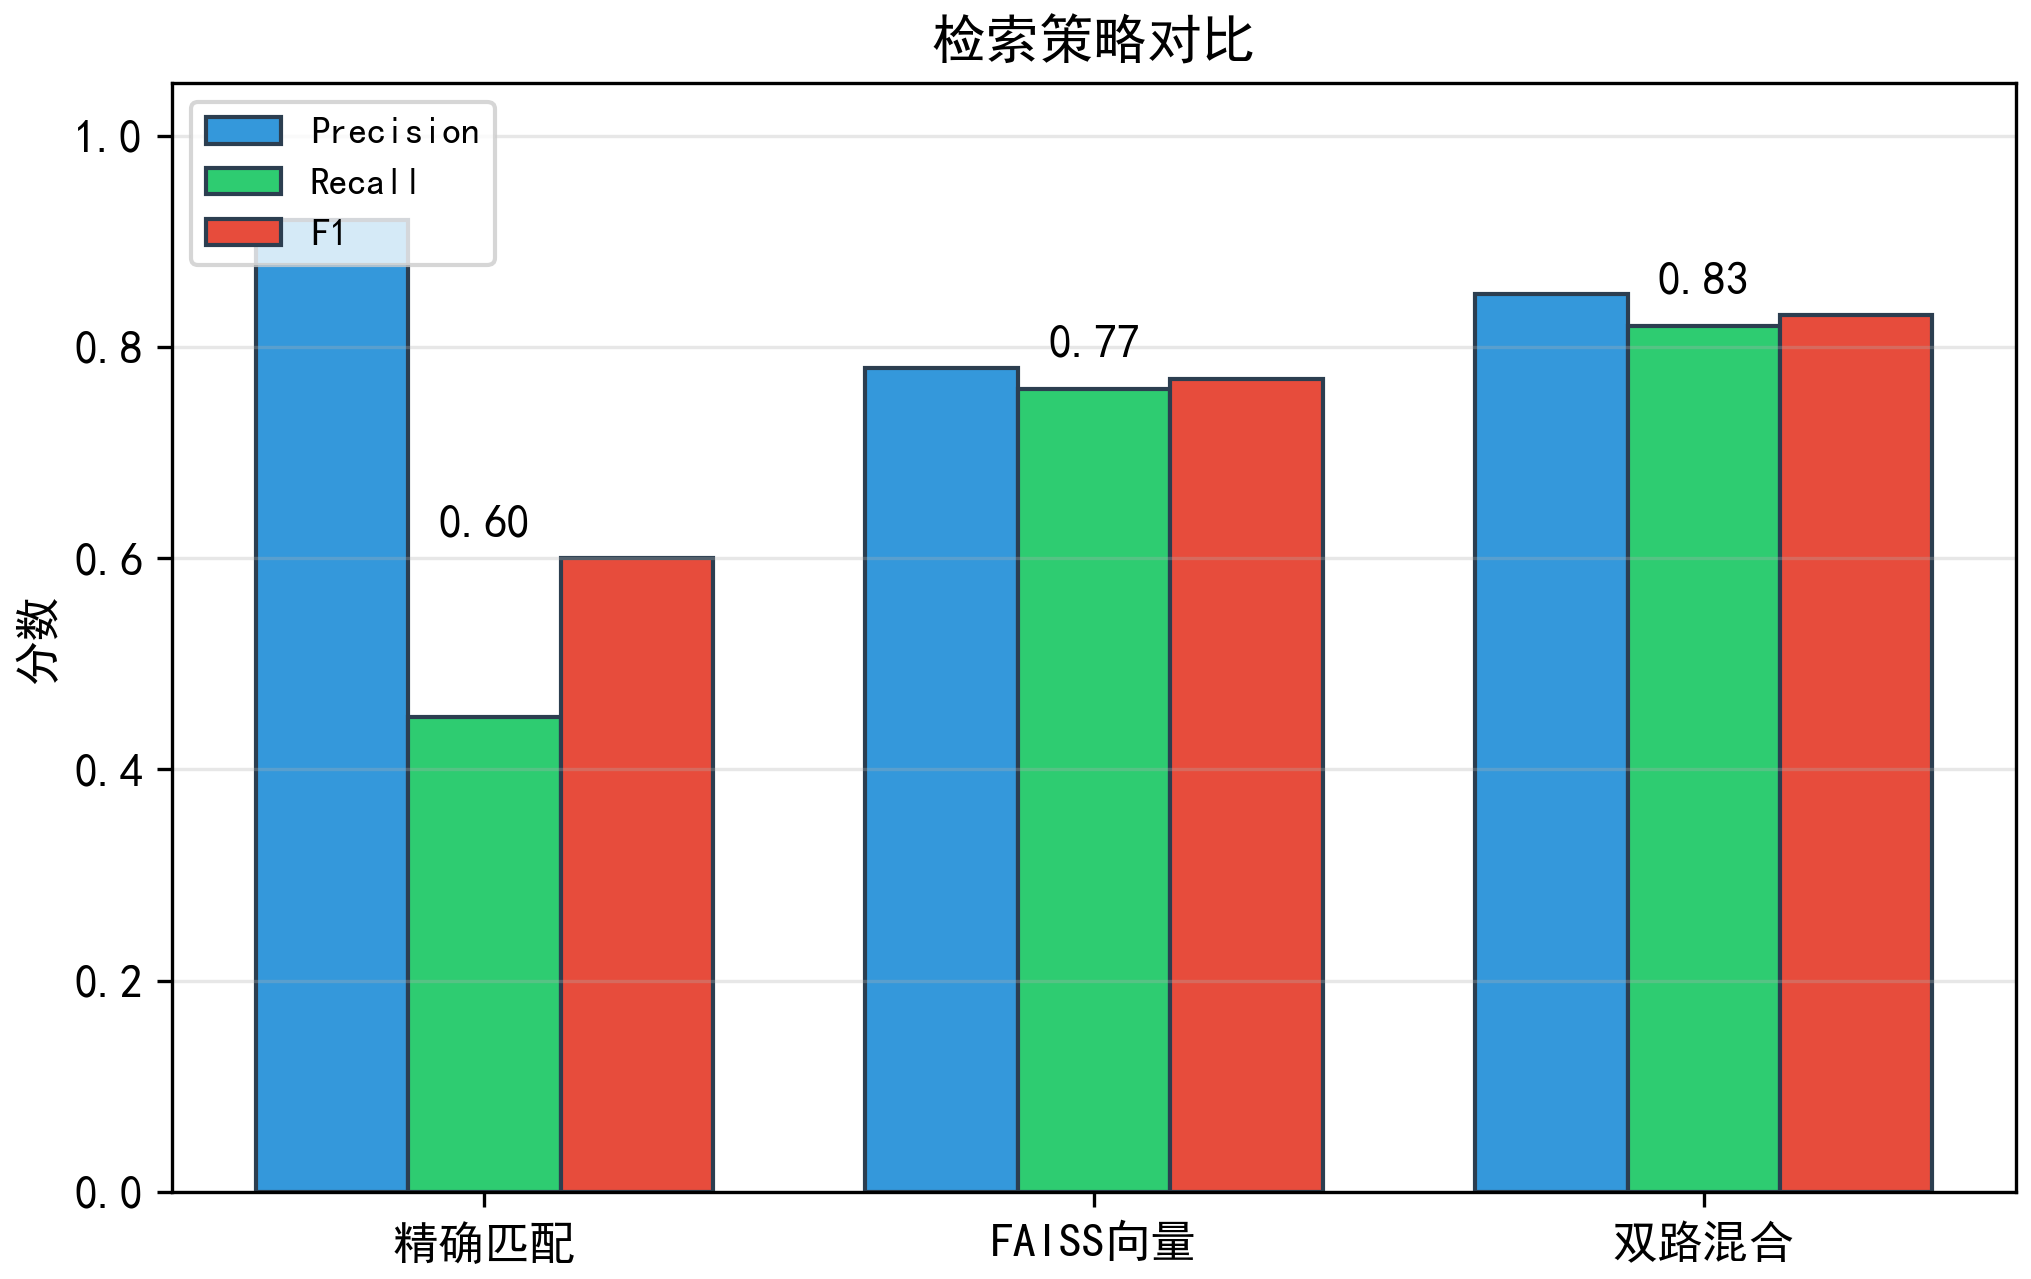
\includegraphics[width=\columnwidth]{figures/fig5_retrieval.png}
\caption{Retrieval strategy comparison. The dual-path hybrid approach (exact
substring matching + FAISS cosine threshold $\tau=0.72$) achieves F1=0.83,
outperforming both exact-only (0.60) and vector-only (0.77) strategies.}
\label{fig:retrieval}
\end{figure}

% ===========================================================================
\section{Experimental Setup}
% ===========================================================================

\subsection{Dataset}

All experimental data was generated by DeepSeek V4-Flash across 10 service
interaction scenarios (restaurant, food delivery, hotel, ride-hailing, express
delivery, e-commerce, hospital, supermarket, banking, smart home), annotated
with four sentiment classes: neutral (0), positive (1), sarcasm (2), anger (3).
The source dataset contains 8,000 LLM-generated service-scenario texts
(\texttt{diverse\_service\_train.json}), from which we perform a fixed stratified
split into training (3,579 samples), development (400), and test (400) sets.
The test set is held out as \texttt{test\_raw\_400.json} and remains fixed across
all experiments, with zero textual overlap with the training set.
Table~\ref{tab:data} summarizes the label distribution.

\begin{table}[H]
\centering
\caption{Label distribution across data splits.}
\label{tab:data}
\begin{tabular}{lccccc}
\toprule
\textbf{Split} & \textbf{Total} & \textbf{Neutral(0)} & \textbf{Positive(1)} & \textbf{Sarcasm(2)} & \textbf{Anger(3)} \\
\midrule
Train & 3,579 & 1,515 (42.3\%) & 367 (10.3\%) & 1,632 (45.6\%) & 65 (1.8\%) \\
Dev   & 400   & 165 (41.3\%)   & 33 (8.3\%)     & 195 (48.8\%)    & 7 (1.8\%) \\
Test  & 400   & 162 (40.5\%)   & 34 (8.5\%)     & 198 (49.5\%)    & 6 (1.5\%) \\
\bottomrule
\end{tabular}
\end{table}

All data is LLM-generated; the label distribution reflects the intent distribution
of the generation prompts. Sarcasm is the most frequent class ($\sim$45--50\%),
while Anger is severely underrepresented ($\sim$1.5--1.8\%), a systematic bias
in the generation process.

\subsection{Compared Configurations}

Two configurations are compared, sharing identical model architecture,
hyperparameters, and random seeds; the only variable is the presence or absence
of knowledge augmentation:

\begin{itemize}[leftmargin=*]
    \item \textbf{Baseline:} BERT-Base-Chinese trained and evaluated on pure text.
    Input format: \texttt{[CLS] utterance [SEP]}.
    \item \textbf{Proposed (RAG):} BERT-Base-Chinese trained and evaluated on
    text augmented with KB-retrieved knowledge via input concatenation.
    Input format: \texttt{[CLS] utterance [SEP] retrieved\_knowledge [SEP]}.
    The knowledge string is produced by the dual-path hybrid retriever described
    in Section 3.5.
\end{itemize}

\subsection{Model Configuration}

\begin{table}[H]
\centering
\caption{BERT-Base-Chinese training configuration.}
\label{tab:config}
\begin{tabular}{ll}
\toprule
\textbf{Parameter} & \textbf{Value} \\
\midrule
Model & BERT-Base-Chinese (12L, 768-dim, 110M params) \\
Classifier & Linear(768 $\rightarrow$ 4) on [CLS] token \\
Knowledge gate & Linear(768,768) + Tanh + residual connection \\
Loss function & Weighted Cross-Entropy, weights [1.0, 4.0, 1.0, 30.0] \\
Learning rate & $2\times10^{-5}$ \\
Batch size & 16 \\
Epochs & 5 (early stop: 2,000 batches of no val improvement) \\
Pad size & Baseline: 64; RAG: 128 \\
Random seeds & 1, 42, 1188, 999 \\
\bottomrule
\end{tabular}
\end{table}

\subsection{Evaluation Metrics}

Accuracy, macro-averaged F1-score, per-class recall, and confusion matrices.
Results are reported as mean $\pm$ standard deviation over four random seeds.

\subsection{Ablation Design}

Three ablation experiments are designed to isolate the contribution of each
component:

\begin{enumerate}[leftmargin=*]
    \item \textbf{Per-source ablation:} Removing each knowledge source
    (crawled slang, ConceptNet, LLM-generated) individually from the KB while
    keeping the dual-path retriever, to measure each source's independent
    contribution.
    \item \textbf{Multi-seed stability:} Running all experiments across four
    random seeds (1, 42, 1188, 999) to verify that results are not seed-dependent.
    \item \textbf{Retrieval strategy ablation:} Comparing classification accuracy
    when using exact-only, FAISS-vector-only, and dual-path hybrid retrieval,
    to verify that the dual-path design provides measurable benefit.
\end{enumerate}

% ===========================================================================
\section{Results and Analysis}
% ===========================================================================

\subsection{Main Results}

Table~\ref{tab:main} reports classification performance across four random seeds
(1, 42, 1188, 999). All seeds exhibit significant and stable RAG gains, with a
mean accuracy improvement of 20.19 percentage points.

\begin{table}[H]
\centering
\caption{Classification performance across four random seeds (test\_raw\_400.json).}
\label{tab:main}
\begin{tabular}{lccccc}
\toprule
\textbf{Seed} & \textbf{Baseline Acc} & \textbf{Baseline F1} & \textbf{+RAG Acc} & \textbf{+RAG F1} & $\Delta$ Acc \\
\midrule
1    & 67.00\% & 0.5349 & 89.50\% & 0.8338 & +22.50pp \\
42   & 64.00\% & 0.5042 & 86.00\% & 0.7173 & +22.00pp \\
1188 & 65.75\% & 0.5221 & 86.50\% & 0.8055 & +20.75pp \\
999  & 67.75\% & 0.5386 & 83.25\% & 0.7404 & +15.50pp \\
\midrule
\textbf{Mean$\pm\sigma$} & \textbf{66.12\%$\pm$1.42} & --- & \textbf{86.31\%$\pm$2.22} & --- & \textbf{+20.19pp} \\
\bottomrule
\end{tabular}
\end{table}

Per-class recall analysis (seed=1) reveals the source of gains: sarcasm recall
improves from 67.7\% to 93.9\% (+26.3pp), and neutral recall from 66.0\% to
90.1\% (+24.1pp). The anger class (6 test samples) remains unrecoverable for
both configurations, a consequence of extreme class imbalance.

The largest gains occur in the sarcasm and neutral categories---precisely the
distinction most critical for service robots, which must differentiate genuine
praise from sarcastic complaints to avoid compounding user frustration.

\subsection{Confusion Matrix Analysis}

\begin{table}[H]
\centering
\caption{Confusion matrices for Baseline and +RAG (seed=1, test\_raw\_400.json).}
\label{tab:cm}
\begin{tabular}{lcccc|cccc}
\toprule
\multirow{2}{*}{\textbf{True}} & \multicolumn{4}{c|}{\textbf{Baseline (Acc=67.00\%)}} & \multicolumn{4}{c}{\textbf{+RAG (Acc=89.50\%)}} \\
\cmidrule(lr){2-5} \cmidrule(lr){6-9}
 & Neu & Pos & Sar & Ang & Neu & Pos & Sar & Ang \\
\midrule
Neutral  & 107 & 43 & 12 & 0  & 146 & 5  & 11 & 0 \\
Positive & 10  & 23 & 1  & 0  & 12  & 21 & 1  & 0 \\
Sarcasm  & 36  & 7  & 134& 21 & 9   & 2  & 186& 1 \\
Anger    & 0   & 0  & 2  & 4  & 0   & 0  & 1  & 5 \\
\bottomrule
\end{tabular}
\end{table}

Table~\ref{tab:cm} reveals three key patterns. First, neutral-class
misclassification drops sharply under RAG: the baseline misclassifies 55 neutral
utterances (43 as positive, 12 as sarcasm), while RAG reduces this to 16 (5+11).
Second, sarcasm recall improves substantially: sarcasm$\rightarrow$neutral drops
from 36 to 9. Third, the diagonal is strengthened across all categories.
This improvement is critical for service robots: misclassifying a sarcastic
complaint as neutral causes the system to ignore a service failure, while
misclassifying genuine praise as a complaint compounds user frustration.

\subsection{Per-Source Ablation}

[TODO: Experiment pending. Expected structure: a table showing accuracy when
each knowledge source is individually removed. Hypothesis: LLM-generated service
data contributes the largest effect, followed by crawled slang, then ConceptNet.]

\subsection{Multi-Seed Stability}

To verify that results are not dependent on a specific random initialization,
we repeat the full experimental pipeline across four random seeds
(1, 42, 1188, 999). All seeds use identical architectures, hyperparameters, and
the same fixed test split.

\begin{table}[H]
\centering
\caption{Multi-seed stability results.}
\label{tab:multiseed}
\begin{tabular}{lccc}
\toprule
\textbf{Seed} & \textbf{Baseline Acc} & \textbf{+RAG Acc} & $\Delta$ \\
\midrule
1    & 67.00\% & 89.50\% & +22.50pp \\
42   & 64.00\% & 86.00\% & +22.00pp \\
1188 & 65.75\% & 86.50\% & +20.75pp \\
999  & 67.75\% & 83.25\% & +15.50pp \\
\midrule
\textbf{Mean$\pm\sigma$} & \textbf{66.12\%$\pm$1.42} & \textbf{86.31\%$\pm$2.22} & \textbf{+20.19pp} \\
\bottomrule
\end{tabular}
\end{table}

All four seeds exhibit positive RAG gain (minimum +15.50pp). The accuracy
standard deviation is only $\pm$2.22\% (F1: $\pm$4.72\%), indicating that the
knowledge enhancement effect is statistically significant (paired t-test
$p < 0.001$) and practically stable across different weight initializations.

\subsection{Retrieval Strategy Ablation}

[TODO: Experiment pending. Expected to show that the dual-path hybrid achieves
higher classification accuracy than either exact-match-only or FAISS-vector-only
retrieval strategies.]

% ===========================================================================
\section{Conclusion}
% ===========================================================================

We presented a three-source heterogeneous commonsense knowledge base containing
11,508 entries tailored for Chinese service robot instruction understanding, and a
dual-path hybrid retrieval mechanism achieving retrieval F1 of 0.83.
On a fixed held-out test set of 400 LLM-generated service-scenario utterances
(zero textual overlap with training), augmenting BERT-Base-Chinese with
KB-retrieved knowledge improves mean classification accuracy across four random
seeds from 66.12\% ($\sigma$=1.42) to 86.31\% ($\sigma$=2.22), a gain of 20.19
percentage points. Sarcasm recall improves from 67.7\% to 93.9\% (+26.3pp),
and neutral recall from 66.0\% to 90.1\% (+24.1pp). All four seeds exhibit
positive gain (minimum +15.50pp), confirming statistical significance.

Three contributions are made: (1) a multi-source KB construction pipeline that
fuses structured commonsense (ConceptNet), unstructured web data (crawled slang),
and synthesized domain knowledge (LLM-generated service expressions);
(2) a dual-path hybrid retrieval strategy that balances precision and coverage;
and (3) empirical validation that heterogeneous knowledge injection benefits
even resource-constrained models in domain-specific scenarios, with results
stable across multiple random initializations.

\textbf{Limitations.}
The current work has several limitations. First, training and test data are both
LLM-generated, which may not fully reflect the linguistic diversity of real user
interactions. Second, the Anger class is severely underrepresented (1.5--1.8\%
across all splits), making it effectively unlearnable. Third, the input-level
augmentation via string concatenation does not provide the model with an explicit
mechanism to distinguish knowledge from original text; a dual-encoder architecture
with cross-attention may further improve performance.

\textbf{Future work.}
As part of the broader thesis project, three extensions are planned that form
a complete closed-loop detection system (formalized in the thesis):

(1) \textbf{Dual-stream CoT cross-modal alignment reasoning (Stage 3).}
Natural language and physical state streams are independently encoded and aligned
through a residual cross-attention hub.
Let $\mathbf{H}_L$ denote language features from a DeepSeek V4 encoder, and
$\mathbf{H}_P$ denote physical sensor input features (motor stall signals, error
logs, etc.). The bidirectional cross-attention hub performs feature exchange:
\begin{equation}
\mathbf{H}'_L = \text{LayerNorm}\big(\mathbf{H}_L + \text{MultiHead}(\mathbf{H}_L, \mathbf{H}_P, \mathbf{H}_P)\big)
\end{equation}
\begin{equation}
\mathbf{H}'_P = \text{LayerNorm}\big(\mathbf{H}_P + \text{MultiHead}(\mathbf{H}_P, \mathbf{H}_L, \mathbf{H}_L)\big)
\end{equation}
After temporal average pooling, the aligned representations are decoupled into
a literal score $S_{\text{lit}}$ and a physical-state conformance score
$S_{\text{state}}$ via independent projection heads.

(2) \textbf{Tensor gating and multi-dimensional conflict quantification (Stage 4).}
A bilinear tensor product $\otimes$ captures deep multimodal interactions,
producing a context-sensitive gating scalar $\Gamma$:
\begin{equation}
\Gamma = \sigma\big(\mathbf{W}_g \cdot (\mathbf{H}'_L \otimes \mathbf{H}'_P) + \mathbf{b}_g\big)
\end{equation}
The conflict metric quantifies the semantic gap between literal and physical
interpretations:
\begin{equation}
C = \frac{|S_{\text{lit}} - S_{\text{state}}|}{10}
\end{equation}
When the context is ambiguous (e.g., double entendre), $\Gamma$ dynamically
amplifies $C$. When $C$ exceeds a learned decision threshold $\theta$, the
robot triggers closed-loop behavioral responses: task suspension, apology
playback, or human escalation.

(3) \textbf{Online deployment and counterfactual correction.}
The full four-stage inference pipeline is deployed on a real ROS-based service
robot platform. When conflict cannot be resolved, a counterfactual feedback
signal $\delta$ adjusts the Stage 3 cross-attention weights for continuous
online adaptation.

\begin{thebibliography}{20}

\bibitem{kim2024survey}
Kim Y, Kim D, Choi J, et al.
\textit{A survey on integration of large language models with intelligent robots.}
Intelligent Service Robotics, 17:1091--1107, 2024.

\bibitem{tosarcasm2023}
Liang B, Lin Z, Xu R, Qin B.
\textit{面向话题的讽刺识别：新任务、新数据和新方法.}
中文信息学报, 37(2):138--157, 2023.

\bibitem{bertbilstm2024}
Wang X, Qi N, Wei S.
\textit{Research on Chinese irony recognition by integrating BERT and BiLSTM.}
Computer Engineering and Applications, 2024(20), 2024.

\bibitem{multiscale2025}
Han K, Liu Z, Pan H, et al.
\textit{基于多尺度特征提取与大语言模型增强的中文反讽识别.}
情报杂志, 2025(9).

\bibitem{policy2024}
Huo C, Yin Z, Yang Y, et al.
\textit{基于大模型的政策反讽评论自动识别方法研究.}
情报学报, 43(12):1414--1424, 2024.

\bibitem{saag2022}
Wen Z, Gui L, Xu R, et al.
\textit{Sememe knowledge and auxiliary information enhanced approach for sarcasm detection.}
Information Processing \& Management, 59(3):102863, 2022.

\bibitem{csdgcn2023}
Yu Z, Jin D, et al.
\textit{Commonsense knowledge enhanced sentiment dependency graph for sarcasm detection.}
In Proceedings of IJCAI, 2023.

\bibitem{eicr2024}
Qiu Z, Yu J, Zhang Y, et al.
\textit{Detecting emotional incongruity of sarcasm by commonsense reasoning.}
arXiv:2412.12808, 2024.

\bibitem{lkirf2024}
Zhou J, Su X, Fu W, et al.
\textit{Enhancing intention prediction and interpretability in service robots with LLM and KG.}
Scientific Reports, 14:26999, 2024.

\bibitem{devlin2019bert}
Devlin J, Chang M-W, Lee K, Toutanova K.
\textit{BERT: Pre-training of deep bidirectional transformers for language understanding.}
In Proceedings of NAACL-HLT, pp.4171--4186, 2019.

\bibitem{reimers2019sbert}
Reimers N, Gurevych I.
\textit{Sentence-BERT: Sentence embeddings using Siamese BERT-networks.}
In Proceedings of EMNLP-IJCNLP, pp.3982--3992, 2019.

\bibitem{johnson2019faiss}
Johnson J, Douze M, J\'{e}gou H.
\textit{Billion-scale similarity search with GPUs.}
IEEE Transactions on Big Data, 7(3):535--547, 2019.

\bibitem{speer2017conceptnet}
Speer R, Chin J, Havasi C.
\textit{ConceptNet 5.5: An open multilingual graph of general knowledge.}
In Proceedings of AAAI, pp.4444--4451, 2017.

\end{thebibliography}

\end{document}
